\section{Expériences}\label{sec:experiences}
\subsection{Protocole}
Toutes les mesures viennent d'une seule exécution de \code{run-all.py} \texttt{-{}-reset} sur le
code final : 19 étapes réussies en 2 h 01, une seule à la fois et avec un seul
déploiement allumé \cite{experiences}. La machine est un Ryzen 5 7600 (6 cœurs, 12 threads)
avec 32 Go de mémoire et un SSD, sous Windows 11. Docker 28.5.1 sur WSL2 voit 12 CPU et
16,4 Go. Les versions sont MongoDB 8.0.16, Python 3.12.10 et l'API compilée pour Java 21,
exécutée sous Java 24.0.1 avec \code{-Xmx768m}. Le cache WiredTiger est fixé à 1,4 Go en
local et à 0,7 Go par shard, pour garder le même cache total ; les conteneurs n'ont pas d'autre limite. Jenkins tournait
aussi sur le PC, sans que nous mesurions sa consommation. Les temps sont ceux vus par un
client HTTP de l'API. Les paramètres exacts de chaque requête sont dans
\chemin{scripts/common.py} et dans les fichiers de résultats.

\subsection{E1 : volume et chargement}
Les jeux sont cumulés et mesurés en local pendant le chargement. Les « trajets distincts »
sont les lignes du profil activity, donc sans montant négatif ni doublon exact. Chaque
latence est la médiane de cinq appels après un échauffement ; l'écart-type le plus grand
vaut 0,67 s.

\begin{center}\small
\begin{tabular}{lrrr}
\toprule
 & 1 mois & 3 mois & 6 mois\\
\midrule
Lignes sources & 2\,964\,624 & 9\,554\,778 & 20\,332\,093\\
Trajets distincts & 2\,929\,120 & 9\,438\,882 & 20\,074\,661\\
Ingestion cumulée (s) & 90,4 & 302,8 & 652,6\\
Données / index (Mo) & 346,7 / 492,9 & 1\,116,2 / 1\,213,8 & 2\,378,0 / 2\,480,5\\
\midrule
F1 JFK, janvier (s) & 1,588 & 1,629 & 1,572\\
F3 Brooklyn, janvier (s) & 12,819 & 11,376 & 11,203\\
F4 JFK $\to$ Midtown, janvier (s) & 0,050 & 0,045 & 0,043\\
F5 Brooklyn, janvier (s) & 0,253 & 0,258 & 0,266\\
F2 Brooklyn, janvier (s) & 2,010 & 8,269 & 19,487\\
\midrule
F1 zone 181, toute la base (s) & 0,017 & 0,056 & 0,163\\
F2 Brooklyn, toute la base (s) & 2,019 & 10,254 & 25,509\\
\bottomrule
\end{tabular}
\end{center}

Chaque mois s'importe à un rythme de 30\,000 à 33\,000 lignes par seconde. Quand la base
est multipliée par 6,9, les requêtes sur janvier de F1, F3, F4 et F5 ne ralentissent pas.
F2 sur janvier est l'exception, avec un temps multiplié par 9,7. Son filtre combine la date
de départ et un \code{$or} sur les zones de départ et d'arrivée. Or l'index d'arrivée
contient la date d'arrivée : il ne borne pas la date de départ, et nous en déduisons que MongoDB relit les arrivées à Brooklyn de toute la base avant de filtrer ; nous n'avons pas enregistré le plan de cette requête. Nous n'avons pas mesuré d'index
corrigé.

À six mois, l'ingestion dure 652,6 s en local, 646,8 s en zone et 783,2 s en période. Les
données pèsent 2,4 Go partout, mais les index passent de 2,5 Go en local à 4,5 Go en zone
et 5,0 Go en période, pour un total de 4,9, 6,9 et 7,4 Go. Nous n'avons établi la cause ni
de ce surcoût d'index ni du chargement plus lent en période.

\subsection{E2 : local et réparti}\label{sec:e2}
Les données sont celles de six mois. Avant chaque série, les serveurs redémarrent, ce qui
vide le cache de MongoDB mais pas le cache disque de la VM. Chaque requête reçoit un premier
appel, un échauffement, puis cinq appels mesurés avec un seul client.

\begin{center}\footnotesize
\begin{tabular}{@{}l*{3}{r}rrr@{}}
\toprule
 & \multicolumn{3}{c}{Médiane en s (écart-type)} & \multicolumn{3}{c}{Milliers de documents lus par appel}\\
\cmidrule(lr){2-4}\cmidrule(l){5-7}
Requête & Local & Zone & Période & Local & Zone s1/s2 & Période s1/s2\\
\midrule
F1 JFK, départs, mars & 1,584 (0,327) & 1,444 (0,202) & 1,808 (0,355) & 158 & 0 / 158 & 158 / 0\\
F1 zone 181, arrivées, semestre & 1,309 (0,050) & 0,790 (0,028) & 0,843 (0,074) & 50 & 23 / 27 & 24 / 26\\
F2 cinq zones, semestre & 5,396 (0,110) & 3,270 (0,049) & 3,524 (0,226) & 190 & 89 / 101 & 87 / 103\\
F2 Brooklyn, trimestre & 20,976 (0,196) & 13,261 (0,169) & 12,545 (0,132) & 818 & 358 / 460 & 397 / 0\\
F3 Brooklyn, mars & 28,008 (1,006) & 19,231 (0,351) & 35,586 (0,370) & 7\,321 & 3\,664 / 3\,657 & 7\,321 / 0\\
F4 JFK $\to$ Midtown & 0,074 (0,025) & 0,095 (0,015) & 0,098 (0,033) & 4 & 0 / 4 & 4 / 0\\
F5 Brooklyn, mars & 1,930 (0,141) & 1,445 (0,039) & 2,762 (0,046) & 92 & 40 / 52 & 92 / 0\\
F5 ville, autour d'avril & 38,145 (0,854) & 21,877 (1,364) & 59,115 (1,501) & 4\,120 & 2\,063 / 2\,057 & 3\,246 / 874\\
\bottomrule
\end{tabular}
\end{center}

Sur une zone ciblée, les écarts restent petits : pour F1 JFK, ils sont du même ordre que
les écarts-types. Sur les requêtes larges, le temps suit le shard le plus chargé. Pour F5
ville, l'\code{explain} donne 54,7 s à shard1 sur les 59,2 s du placement par période, où ce
shard lit 3\,246 milliers de documents. Le placement par zone coupe la lecture en deux
parts égales et gagne 43\,\% sur le local. Le CPU total des instances pour les cinq appels
vaut 209 s en local, 220 s en zone et 344 s en période.


\begin{itemize}
\item \textbf{Parallélisme.} Sur F2 cinq zones, les deux shards lisent les mêmes documents
que le local à eux deux. Le temps baisse de 39\,\% en zone et le CPU total reste presque
stable (30,2 s puis 31,1 s).
\item \textbf{Cache réduit.} Sur F3 et F5 Brooklyn en période, seul shard1 lit, et il lit
autant que le local, avec 0,7 Go de cache au lieu de 1,4. Les temps augmentent de 27\,\% et
43\,\%, alors que \code{mongos} consomme au plus 0,25 s de CPU. Sur F5 ville, le CPU par
document vaut 10,1 µs en local et 10,6 µs en zone, où le rapport entre documents et cache
est le même, contre 18,9 µs sur shard1 en période, qui lit 1,6 fois plus pour le même cache.
Le cache est la cause probable, mais nous n'avons pas relevé de compteur d'éviction.
\item \textbf{Données réduites.} Sur F2 Brooklyn en période, shard1 lit 397 milliers de
documents contre 818 ailleurs. Comme il ne contient que janvier--mars, l'index d'arrivée
n'y trouve que ces trajets (voir E1). Le gain de 40\,\% vient donc de cette réduction et
pas d'un parallélisme : shard2 ne lit rien.
\end{itemize}
Le premier appel après redémarrage coûte peu : F5 ville prend 38,6 s contre 38,1 s en local,
F1 JFK 2,6 s contre 1,6 s. Ces temps n'ont pas la valeur d'une vraie lecture à froid, puisque
le cache disque de la VM reste plein.

\subsection{E3 : charges contrastées}
La charge A vise quatre zones très actives (F1 au départ et F4 sur une semaine). La charge B
couvre des zones et des périodes variées (F1 à l'arrivée sur le semestre, F2 sur quatre
semaines, F5 avec cinq semaines d'historique, sur Brooklyn et Queens). Chaque mélange compte
60 requêtes envoyées par trois clients, après une passe d'échauffement. La graine est fixe :
un mélange rejoue les mêmes requêtes sur chaque déploiement, mais pas celles d'un autre
mélange. Il n'y a eu qu'un passage par mélange et aucune erreur : la table ne donne donc pas
de variabilité, et nous lisons comme une égalité les écarts de quelques pour cent.

\begin{center}\footnotesize
\begin{tabular}{@{}lrrrrrrrrrrr@{}}
\toprule
 & \multicolumn{3}{c}{Durée totale (s)} & \multicolumn{3}{c}{Médiane A (s)} & \multicolumn{3}{c}{Médiane B (s)} & \multicolumn{2}{c}{CPU s1 / s2 (s)}\\
\cmidrule(lr){2-4}\cmidrule(lr){5-7}\cmidrule(lr){8-10}\cmidrule(l){11-12}
A / B & Local & Zone & Pér. & Local & Zone & Pér. & Local & Zone & Pér. & Zone & Pér.\\
\midrule
60 / 0 & 9,5 & 7,9 & 17,0 & 0,496 & 0,418 & 0,608 & --- & --- & --- & 9 / 12 & 38 / 12\\
42 / 18 & 71,9 & 50,9 & 50,5 & 0,574 & 0,656 & 0,677 & 2,524 & 1,984 & 2,207 & 101 / 130 & 98 / 83\\
18 / 42 & 153,6 & 102,4 & 104,1 & 0,410 & 0,442 & 0,701 & 7,947 & 5,461 & 5,704 & 230 / 276 & 163 / 169\\
0 / 60 & 203,4 & 146,2 & 135,6 & --- & --- & --- & 7,287 & 6,020 & 6,439 & 355 / 425 & 190 / 311\\
\bottomrule
\end{tabular}
\end{center}

\begin{figure}[!htbp]\centering
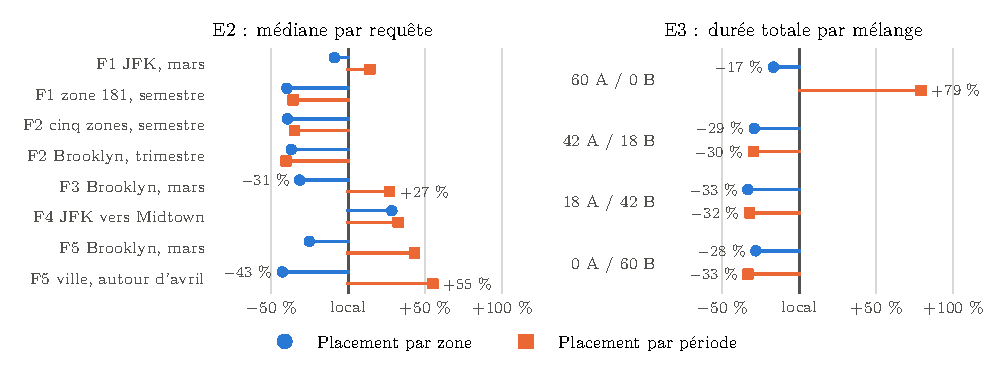
\includegraphics[width=\linewidth]{figures/temps-par-rapport-au-local.pdf}
\caption{Écart de temps de chaque placement par rapport au serveur local : à gauche du trait « local », le placement est plus rapide. Sur F4 et F1 JFK, l'écart reste petit en valeur absolue ou proche de la variabilité.}\label{fig:temps}
\end{figure}

Nous avons écrit la prédiction avant les mesures \cite{prediction}.
\begin{itemize}
\item \textbf{Faux : le local est le plus rapide sur A.} Le placement par zone termine en
7,9 s contre 9,5 s. Nous attendions un surcoût de \code{mongos} et du cache coupé en deux.
Or \code{mongos} consomme 0,3 s de CPU, et les zones chaudes sont séparées (568 et 797
milliers de documents) : la charge ne se concentre pas sur un shard. Le local garde une
médiane A un peu plus basse dans les deux mélanges intermédiaires.
\item \textbf{Juste, avec une erreur d'ampleur : la zone est le meilleur placement réparti
sur A.} Nous attendions un écart faible, et il va du simple au double (7,9 s contre 17,0 s).
Les 12 appels F4 dont toute la fenêtre tombe sur shard1 prennent 1,3 à 3,0 s en période, contre
au plus 0,65 s pour les 17 autres et jamais plus de 0,58 s en zone. Sur tout le mélange, shard1 lit 6,8 millions
de clés pour 1,1 million de documents. Le même F4 n'était pas lent dans E2 (0,098 s). Nous n'avons pas enregistré les plans pendant E3 : un mauvais choix d'index sur shard1 reste une hypothèse.
\item \textbf{Juste : le réparti gagne 20 à 40\,\% sur B.} La durée baisse de 28\,\% en zone et
33\,\% en période.
\item \textbf{Faux : F1 reste plus lent en réparti à cause de \code{$facet}.} Dans E2, F1 sur la
zone 181 descend de 1,309 s à 0,790 et 0,843 s. La lecture, faite en parallèle avant la fusion,
semble peser plus que \code{$facet}.
\item \textbf{À moitié juste : la période bat la zone sur B.} Elle gagne en durée totale (135,6 s
contre 146,2 s), mais pas en médiane (6,439 s contre 6,020 s). Sa durée profite des F2 longs,
médiane 12,8 s contre 15,2 s. Elle lit aussi moins de documents, 19,3 millions contre 25,4.
\item \textbf{Faux : le meilleur choix bascule du local au réparti au milieu du mélange.} Le
local ne gagne aucun mélange en durée totale (figure~\ref{fig:temps}) : la zone est devant dès 60 / 0, et zone et période
sont à égalité dans les deux mélanges intermédiaires.
\item \textbf{Juste : la charge est déséquilibrée en période quand les requêtes visent un
trimestre.} Sur A, shard1 consomme 38 s de CPU et shard2 12 s, contre 9 et 12 s en zone.
\end{itemize}

En zone, le temps gagné se paie en ressources. Sur 0 / 60, le CPU total passe de 628 s en local à
787 s, \code{mongos} compris ; il descend à 508 s en période, qui lit moins. Le serveur local
émet 168 Mo ; les shards en émettent 1\,231 en zone et 1\,094 en période, à cause des
résultats partiels et de la fusion. La mémoire relevée à la fin passe de 2,2 Go à 2,7 Go.

Pour des requêtes ciblées fréquentes et des analyses de la ville occasionnelles, nous
retiendrions le placement par zone : il arrive premier ou à égalité sur trois mélanges sur quatre,
il répartit le travail de façon régulière et il évite les 59 s de F5 ville. Il perd 7\,\% face
à la période sur 0 / 60 et coûte 42\,\% de stockage de plus que le local. Nous n'avons pas réalisé l'expérience bonus E4.
